\question \textbf{Rook at This}\newline
Given the chessboard below, imagine we place 7 rooks on random squares. What is the probability that all of these rooks are safe from each other? (No need to simplify!)

Note: If a rook is placed at square $(i,j)$, no pieces in column $j$ or row $i$ are “safe”. 
\begin{solution}
Consider the process of placing each rook on the board. When we place rook 1, we eliminate an entire row and an entire column, so we have effectively restricted the chessboard to a (disjoint) 7x7 board. Each time we add a piece, we lose a row/column. So after the 7th piece is placed, we have just a 1x1 board left. 

We can count the ways to set up such a scenario using the multiplication rule: 
\[N = 8^2 * 7^2 * 6^2 \dotsc * 2^2\]

The total number of ways we could have placed 7 pieces on a 64 square board is $D = {64 \choose 7} * 7!$ (since the order in which we place the rooks matters based on our process above). Our final answer is then $\frac{N}{D}$

\end{solution}

\begin{center}
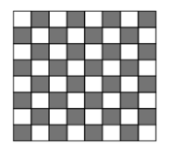
\includegraphics{rook.jpg}
\end{center}